\chapter{Experimenteller Aufbau}\label{cha:experimentAufbau}
\section{Versuchsanordnung}\label{sec:versuchsanordnung}

Wie schon in \autoref{sec:versuchsTheorie} besprochen, beruht das Millikan-Experiment auf dem Kräftegleichgewicht von Gewichtskraft und elektrischer Kraft. Zuerst wird ein dunkler Raum gebraucht. Am Besten funktioniert es mit einer Dunkelkammer, in der kein Licht ist. Das einzige Licht, das gebraucht wird ist Mikroskoplicht am Experimentapparat. Es werden während dem Experiment sehr kleine Öltröpchen mit einem Zerstäuber in eine Kammer gesprüht. Danach wird anhand des Lichtes und dem Mikroskop die Fallgeschwindigkeit des Tröpfchens gemessen. Der Boden und die Decke der Kammer, bestehen aus elektrischen Kapazitoren. Das bedeutet, die Kammer kann ein elektrisches Feld erzeugen. Mit einem Schalter kann die Richtung des elektrischen Feldes gewechselt werden. Diese Funktion wird bei der zweiten Messung gebraucht. Da werden die Kapazitoren eingeschaltet, so dass das elektrische Feld nach oben zeigt (Decke + Boden -). Wenn die Tröpfchen negativ geladen sind, werden sie die Schwerkraft überwinden können und werden nach oben steigen. Dabei wird wieder die Geschwindigkeit gemessen, die die Tröpchen brauchen, um von einer Linie des Gitters zur anderen zu kommen. Diese ganze Prozedur wiederholt man, bis das Tröpfchen nicht mehr gesehen werden kann. Eine schöne Schritt-für-Schritt Anleitung wird in \autoref{sec:durchfuehrung} gezeigt.

\section{Material}\label{sec:material}

In dieser Arbeit wurde das \textit{Model AP-8210 von PASCO scientific} mit der Halogenlampe verwendet. \\

\noindent \textbf{Material, das dabei ist:}

\begin{itemize}
	\item Apparat Plattform und Kondensator Ladungsschalter (Eine genauere Beschreibung der Plattform in \autoref{sub:inhaltApparatur})
	\item 12 Volt DC Transformator für die Halogen Lampe
	\item nicht flüchtiges Öl
	\item Ölsprüher 
\end{itemize}

\subsection{Plattform}\label{sub:inhaltApparatur}
Da das Experiment schon fertig gebaut ist, werden jetzt alle Komponenten aufgezählt, die sich auf der Plattform befinden.

\noindent \textbf{Komponenten Plattform:}

\begin{itemize}\label{item:apparatur}
	\item Tröpfchenbetrachtungskammer (Wird im nächsten \autoref{sub:viewingChamber})
	\item Betrachtungsfernrohr (30X, Hellfeld, aufrechtes Bild) mit Fadenkreuz (Linienabstand: 0,5 mm große Teilung, 0,1 mm kleine Teilung), Fadenkreuz-Fokussierring und Tropfenfokussierring
	\item Halogen Lampe (12 V, 5 W)
	\item Fokussierdraht
	\item Kondensatorenspannungs Anschlüsse
	\item Thermistor Anschlüsse (sind an den unteren Kondensator eingebaut)
	\item Thermistor Tabelle (Widerstand-Temperatur)
	\item Ionisationsquellen Schalter (3 verschiedene Positionen: Ionisation AN, Ionisation AUS, Sprüh Position)
	\item Wasserwaage
	\item Kondensator Ladungsschalter (mit einem Meter Kabel, um Vibrationen aus dem Weg zu gehen)
\end{itemize}


\subsection{Betrachtungskammer}\label{sub:viewingChamber}
Die Betrachtungskammer kann auseinandergenommen werden. Die einzelnen Komponenten werden hier aufgelistet.

\noindent \textbf{Einzelteile der Betrachtungskammer:}

\begin{itemize}\label{item:betrachtungskammer}
	\item Deckel
	\item Gehäuse
	\item Tröpfchenlochabdeckung
	\item obere Kondensatorplatte
	\item Abstandshalter aus Plastik (ungefähr 7.6mm dick)
	\item untere Kondensatorplatte
	\begin{itemize}
		\item Thorium-232 Alphateilchenquelle
		\item elektronische Verbindung zur oberen Platte
	\end{itemize}
	\item konvexe Linse
\end{itemize}

\begin{figure}[h]
	\centering
	\begin{minipage}[t]{0.45\textwidth}
		\centering
		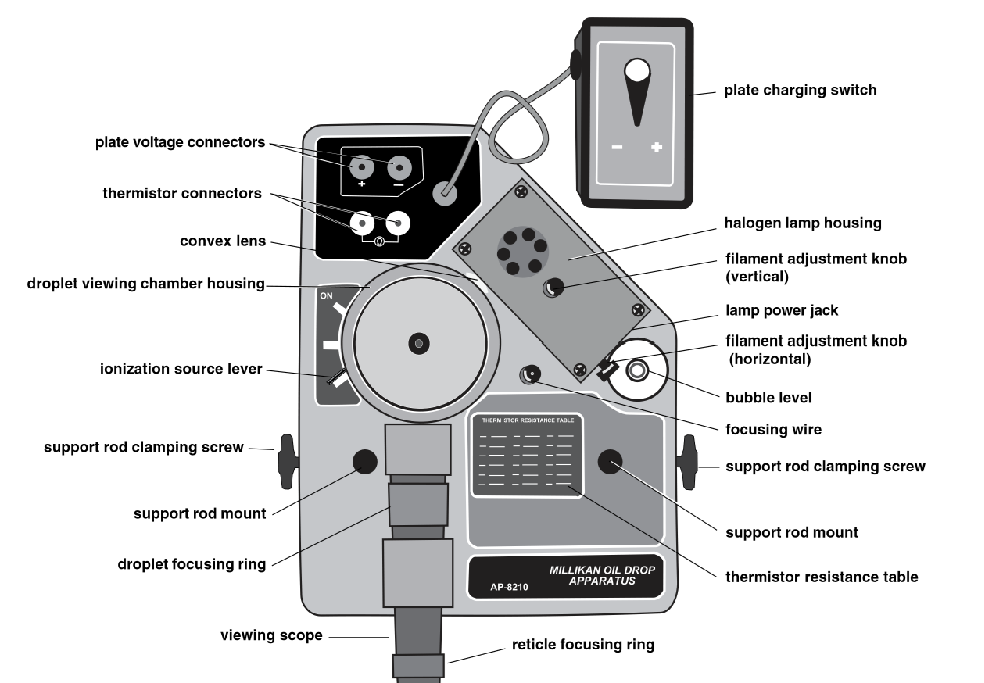
\includegraphics[scale=0.5]{bilder/pdf/plattformKomponenten.pdf}
		\caption{Komponenten der Plattform}
		\label{fig:plattformKomp}
	\end{minipage}
	\hfill
	\begin{minipage}[t]{0.45\textwidth}
		\centering
		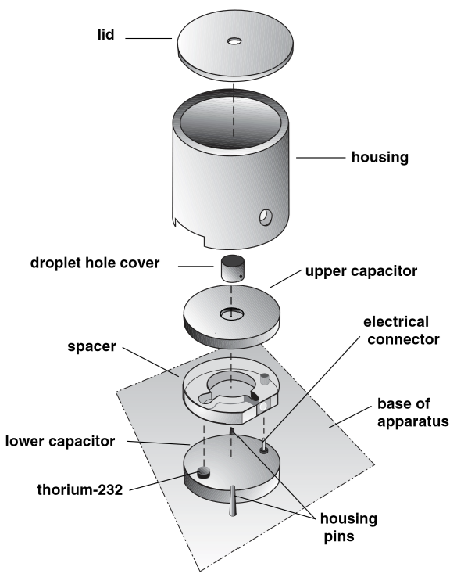
\includegraphics[width=\textwidth]{bilder/pdf/BetrachtungsKammerKomponenten.pdf}
		\caption{Komponenten der Betrachtungskammer}
		\label{fig:betrachtKomp}
	\end{minipage}
\end{figure}





